\documentclass[12pt, a4paper]{article} 
\usepackage[utf8]{inputenc}
\pagestyle{plain} 
\usepackage{pdflscape}
\usepackage[slovak]{babel}
\usepackage[dvipdf]{graphicx}
\usepackage[letterpaper, margin=2cm]{geometry}
\title{Dokumentácia projektu IFJ}
\author{Svätopluk Hanzel, Samuel Hulla, Tomáš Haas}
\date{9.12.2016}


\begin{document}
    \begin{titlepage}
        \begin{center}
        {\scshape\LARGE Vysoké učení technické v Brně \par}
        {\Large Fakulta informačních technologií\par}
        \vspace{3cm}
        {\scshape\LARGE Dokumentácia projektu IFJ\par}
        {\Large Interpret Jazyka IFJ16 \par}
        \vfill
        {\Large Tým 003, Varianta a/2/I}\\
        Rozšírenia: FUNEXP, BASE, BOOLEAN\\
        \vspace{1cm}
        \textbf{Svätoplik Hanzel(xhanze10)} - 20\% \\
        Tomáš Haas(xhaast00) - 20\% \\
        Samuel Hulla(xhulla00) - 20\% \\
        Matúš Juhász(xjuhas02) - 20\% \\
        Dominik Križka(xkrizk02) - 20\% \\
        \vspace{1cm}
        {\hfill Brno, 22.12.2016}
        \end{center}
    \end{titlepage}
    
    \tableofcontents{}
    \newpage
    \setcounter{page}{1}
    \section{Úvod}
    Táto dokumentácia slúži ako textová časť riešenia projektu z predmetu IFJ pre rok 2016/2017. Celý dokument sa delí do niekoľkých kapitol a príloh. Postupne sú rozoberané všetky dôležité prvky implementácie jednotlivých častí interpretu
    \newpage
    \section{Práca v tíme}
     Zo začiatku projektu bola v našom tíme snaha o pravidelne stretnutia 1-2-krát týždenne. To sa však postupne ukázalo ako neefektívne vzhľadom na malé množstvo užitočných informácii, ktoré sa prebrali počas týchto stretnutí a tak sa celá komunikácia presunula na Slack a skôr sa rozdelila medzi ľudí spolupracujúcich na jednotlivých častiach projektu.Tým pádom sa často stalo, že na jednotlivých častiach projektu sa pracovalo skôr skupinovo ako individuálne \\
	 Rozhodnutia o smerovaní projektu boli síce centralizované, ale zároveň otvorené k diskusii.        
        \subsection{Verzovací systém}
			Ako nástroj na správu verzií a zdielanie kódu sme zvolili GIT, pričom vzdialený ako vzdialený repozitár bol zvolený privátny server GitLab, ktorý zároveň slúžil na zadávanie tzv. \texttt{issues} , teda problémov, ktoré treba vyriešiť.
		\subsection{Rozdelenie práce}
			Vzhľadom na agilný vývoj interpretu sme v našom tíme nemali presne stanované rozdelenie práce podľa rozdelenia interpretu. Na správu úloh sme používali tzv. \texttt{issue tracking} systém, ktorý je súčasťou GitLab serveru.
        \subsection{Automatizované testy}
	        Nevyhnutnou súčasťou takéhoto projektu sú automatizované testy. Napriek iniciatíve a snahe o ich včasné napísanie sa tak bohužial stalo až v poslednej tretine riešenia projektu. Napriek tomu nám však veľmi pomohli pri odhaľovaní chýb.\\
	        Okrem automatizovaných testov sme pre odhaľovanie chýb používali aj nástroje na statickú analýzu kódu.
	\newpage
	\section{Riešenie interpretu}
    V tejto kapitole bude detailne rozobraný postup pri tvorbe, správenie sa a optimalizácia našeho interprétu. Jednotlivé problematiky sú rozdelné do viacero častí, kde sa každej budeme podrobnejšie venovať. 
    
        \subsection{Lexikálna analýza}
        Keď sme začali riešiť lexikálnu analýzu, museli sme si najprv uvedomiť, ako budeme rozlišovať jednotlivé znaky. Rozhodli sme sa, že najpraktickejśie riešenie bude implementovať  \textbf{scanner}. Ten spracúvava jednotlivé znaky - \textbf{tokeny} a rozdeľuje ich do jednotlivých \textbf{stavov} ktoré môžu nastať. 
        
        Aj keď z hľadiska samotnej funkčnosti spracúvavame celý súbor a až potom vyhodnocujeme chyby, z lexikálneho hľadiska by sme mohli naraziť na syntaktickú chybu predtým ako by sme narazili ešte na lexikálnu.Z tohoto dôvodu prioritizujeme postup, kde ideme po jednolitvých tokenoch a skúmame, či je lexikálne všetko v poriadku. V prípade, že nie, dostaneme sa do stavu \verb|SS_LEX_ERROR|.
        
        Presný postup samotného vyhodnocovania je relatívne komplikovaný a zdĺhavý a z toho dôvodu je aj spracovaný vo forme konečného automatu (\ref{sec:KA}) na strane \pageref{sec:KA}
        
        \subsection{Syntaktická a semantická analýza}
        Naša analýza prebieha dvojfázovo, v tej prvej časti sa venujeme \textbf{syntaktickej} časti, nasledovne sa upriamime na lokálne premenné, najprv v hlavnom tele programu a potom aj v jednotlivých funkciách, ktorú riešime pomocou \textbf{tabuľky symbolov}. 
        
        Po bezproblémovom prechode sa môžeme presunúť na semantickú časť. Semantické chyby môžu nastať aj keď je program syntakticky v poriadku, napr. volanie neexistujúcej funkcie, alebo aj existujúcej, ale so zlým počtom parametrov, prípadne volanie neexistujúcich premenných, mylné priradenie hodnoty namiesto logického operátora atď.. 
        
        Zároveň sa v druhej časti generujú inštrukcie pre interpret s ktorými bude potom narábať.
        \newpage
        \subsection{Interpretácia}
        Jedná sa o záverečnú - finalizačnú časť projektu, ktorá prebehne až po vykonaní lexikálnej, syntaktickej a sémantickej analýze. Ak zistíme, že je všetko v poriadku, môžeme začat s interpretovaním.
        
        Pomocou troj-adresového kódu, ktorý využíva  vytvorenú \textbf{sadu inštrukcií} zisťujeme chovanie nášho interpréta. Pri cykloch sme namiesto jednotlivých inštrukcií využila skoky, aby sme zlepšili efektivitu programu. 
        
        Dostávame inštrukciu \verb|IC_EVAL| ktorá volá funckiu \verb|evaluate_expression()|, kde následne rozlišujeme aritmetické a logické operácie a určí výslednú hodnotu výrazu. 
        
        Je dôležité upozoniť, že samotná interpretácia prebieha za behu. Interprét spracúva jednotlivé inštrukcie lineárne a vyhodnocuje ich, až kým všetko neprejdeme a dostaneme náš žiadaný výsledok
        
        \subsection{Algoritmy}
			\subsubsection{Knuth-Morris-Prattův algoritmus}
				Jedná se o algoritmus pro vyhledání podřetězce v řetězci. Klasické (triviální) vyhledávání podřetězce – tedy když postupně procházíme řetězec a u každého znaku zjišťujeme, zda se shoduje s podřetězcem, a v případě neshody se posuneme na další znak a musíme porovnávat s podřetězcem zase od začátku – vede v nejhorším případě až na časovou složitost \textbf{O(m·n)}, kde \textbf{m} je délka řetězce a \textbf{n} délka hledaného podřetězce. Tento algoritmus je tedy velmi neefektivní. O(m+n), tedy je mnohem rychlejší. KMP algoritmus dokáže sledovat, zda se v hledaném podřetězci opakují určité skupiny znaků (podřetězce). Při procházení textu pak při neshodě zjistí, zda se v části podřetězce, která už byla zkontrolována (dokud nedošlo k neshodě), nachází sufix, který je shodný s prefixem.\\
				\textbf{Př.:}\\
				Hledaný podřetězec je \textbf{abcxyabcijk}. Uvažujme, že při procházení textu nastane neshoda až na znaku \textbf{c}. Část podřetězce, která podmínkou prošla, je tedy \textbf{abcxyabc}. V této části je skupina znaků \textbf{abc}, která se opakuje, a to tak, že je zároveň jejím prefixem i sufixem.
				Pokud se v podřetězci nachází taková skupina znaků, při neshodě se pak nemusí začínat znovu od začátku podřetězce a v řetězci se nemusíme vracet zpět ke znaku, od kterého jsme začínali kontrolovat. Protože (opět uvažujme uvedený příklad) pokud jsme prošli podřetězcem bez problému až po \textbf{i}, jsme si jistí, že v procházeném textu jsou předchozí tři znaky \textbf{abc}, což se shoduje s prvními třemi znaky, které bychom hledali, pokud bychom procházeli podřetězec znovu od začátku. Můžeme tedy tyto tři znaky přeskočit a pokračovat dále.
				Nejdříve je nutné projít podřetězec a vytvořit pole (v naší funkci pojmenované fail), do kterého se zapíšou hodnoty podle toho, kolika-znakové skupiny se v podřetězci opakují. Tyto hodnoty pak určují, na kterou pozici v podřetězci se musíme vrátit v případě neshody (tedy i kolik znaků v řetězci již můžeme přeskočit).\\
				\textbf{Př.:}\\\\
				\begin{center}
					\begin{tabular}{|c|c|c|c|c|c|c|c|}
						\hline 
						a & b & c & d & a & b & c & a \\ 
						\hline 
						0 & 0 & 0 & 0 & 1 & 2 & 3 & 1 \\ 
						\hline 
					\end{tabular}\\
				\end{center}
				Algoritmus KMP pak prochází postupně řetězec a porovnává jednotlivé znaky se znaky podřetězce. V případě neshody se pak podle hodnoty v tabulce fail posune na určitou pozici v podřetězci a znaky před touto pozicí již nemusí znovu kontrolovat.
				Výsledkem je algoritmus pracující se složitostí \textbf{O(m+n)}, jelikož při porovnání textu se algoritmus nikdy nevrací, celý ho tedy projde se složitostí O(m), ale předtím je nutné tzv. Předzpracování – vytvoření tabulky fail, což znamená projít podřetězec se složitostí O(n).
				
			\subsubsection{Heapsort algoritmus}
				Řazení haldou/hromadou je velmi efektivní řadící algoritmus, který pracuje s časovou složitostí \textbf{O(n·logn)}, která je však zaručená. Jeho použití je tedy někdy vhodnější než použití quicksortu, který může být v některých případech rychlejší, ale v nejhorších případech dosahuje až složitosti \(O(n^2)\).
				Tento algoritmus řadí pole, které má strukturu binární hromady. Hromada je struktura stromového typu, pro kterou platí, že mezi otcovským uzlem a všemi jeho synovskými uzly je vždy stejná relace (např. otec vždy větší než jeho synové). Binární hromada je založena na binárním stromu.
				Pro hromadu implementovanou jako pole (tedy v našem případě řetězec) platí, že otcovský uzel na indexu i má vždy levého syna na indexu \textbf{2i} a pravého syna na indexu \textbf{2i+1}.
				V každém kroku řazení dojde k porušení struktury a je potřeba se stromem tzv. „zatřást“ (shiftdown), čímž se struktura hromady obnoví.
				Tím se dostane na vrchol hromady prvek podle určitého pravidla (např. největší nebo nejmenší). Pokračujeme tak, že vrchol haldy „utrhneme“ a vložíme ho na další pozici již seřazeného řetězce. Poté pracujeme s haldou o jeden prvek menší, musíme ji znovu opravit (pomocí siftdown) a tento postup opakujeme, dokud má halda nějaké prvky.
				Výsledkem je algoritmus se složitostí \textbf{O(n·logn)}. Operace shiftdown, neboli rekonstrukce hromady, totiž pracuje se složitostí O(logn), je tedy schopná rychle najít extrém v daném poli. Heapsort je algoritmus nestabilní, což znamená, že může dojít k prohození prvků se stejnou hodnotou a že dochází k přesouvání prvků velkými skoky, a je nepřirozený, což znamená, že nehraje žádnou roli fakt, zda bylo pole před začátkem řazení již částečně seřazené.
				
			\subsection{Tabulka symbolů}	
				Je tvorená pomocou binárného vyhladávacieho stromu. Jeho výhodou je, že sú v ňom prvky zoradené tak, že klúče všetkých uzlov lavého podstromu 
				sú menšie ako klúč uzlu a klúče pravého podstromu sú väčšie ako klúč uzlu. To ulahčuje vyhladávanie a nájdeniu prvku je rýchlejšie. 
				Nevýhodou je, že musíme prvky udržovat usporiadané, to znamená, že ak chceme vložit nový prvok, musí být vložený presne tam, kam podla 
				svojej velkosti patrí.
				
				V binárnom strome máme uložené názvy symbolou ich data, ich typ a konkrétne id. Naša implementácia je napísaná rekurzívne. Pre vkladanie nových symbolov sa využíva funkcia \textit{table insert symbol}. Ktorá využíva funkciu \textit{tree insert} pre prácu so binárnym stromom sa využíva aj funkcia \textit{tree search} ktorý vyhladáva na základe zadaného kluča.Po skončení práce sa pomocou funkcie \textit{tree dispose} . Pre naše potreby sme potrebovali hlbkovú kopiu nášho binárneho stromu a z toho dôvodu vznikla funkcia \textit{tree copy} .
    \newpage
	\section{Prílohy}
        \subsection{Konečný automat lexikálneho analyzátora} \label{sec:KA}
        Náš samotný lexiálny analyzátor \texttt{scanner} sa prepína medzi rozlišnými stavmi, podľa toho aké tokeny postupne číta a rozhoduje sa medzi nimi. Po každom možnom stave vyhodnocujeme aký ďaľší môže nastať, prípadne hlásime lexikálnu chybu, keďže sme prečítal znak, ktorý za žiadnych okolností nesmieme dostať v danom stave. 
        
        Týmto spôsobom postupne eliminujeme všetkz možnosti a zo začiatočného bodu \textbf{start} sa postupne dostaneme až do finálneho stavu, ktorý je vyhodnotením a spracovaním spracovaného vstupu, prípadne hlásenie lexikálnej chyby \verb|SS_LEX_ERROR|. Vďaka daným vlastnostiam ho môžeme zakresliť aj vo forme konečného automatu.
        
            \begin{center}
            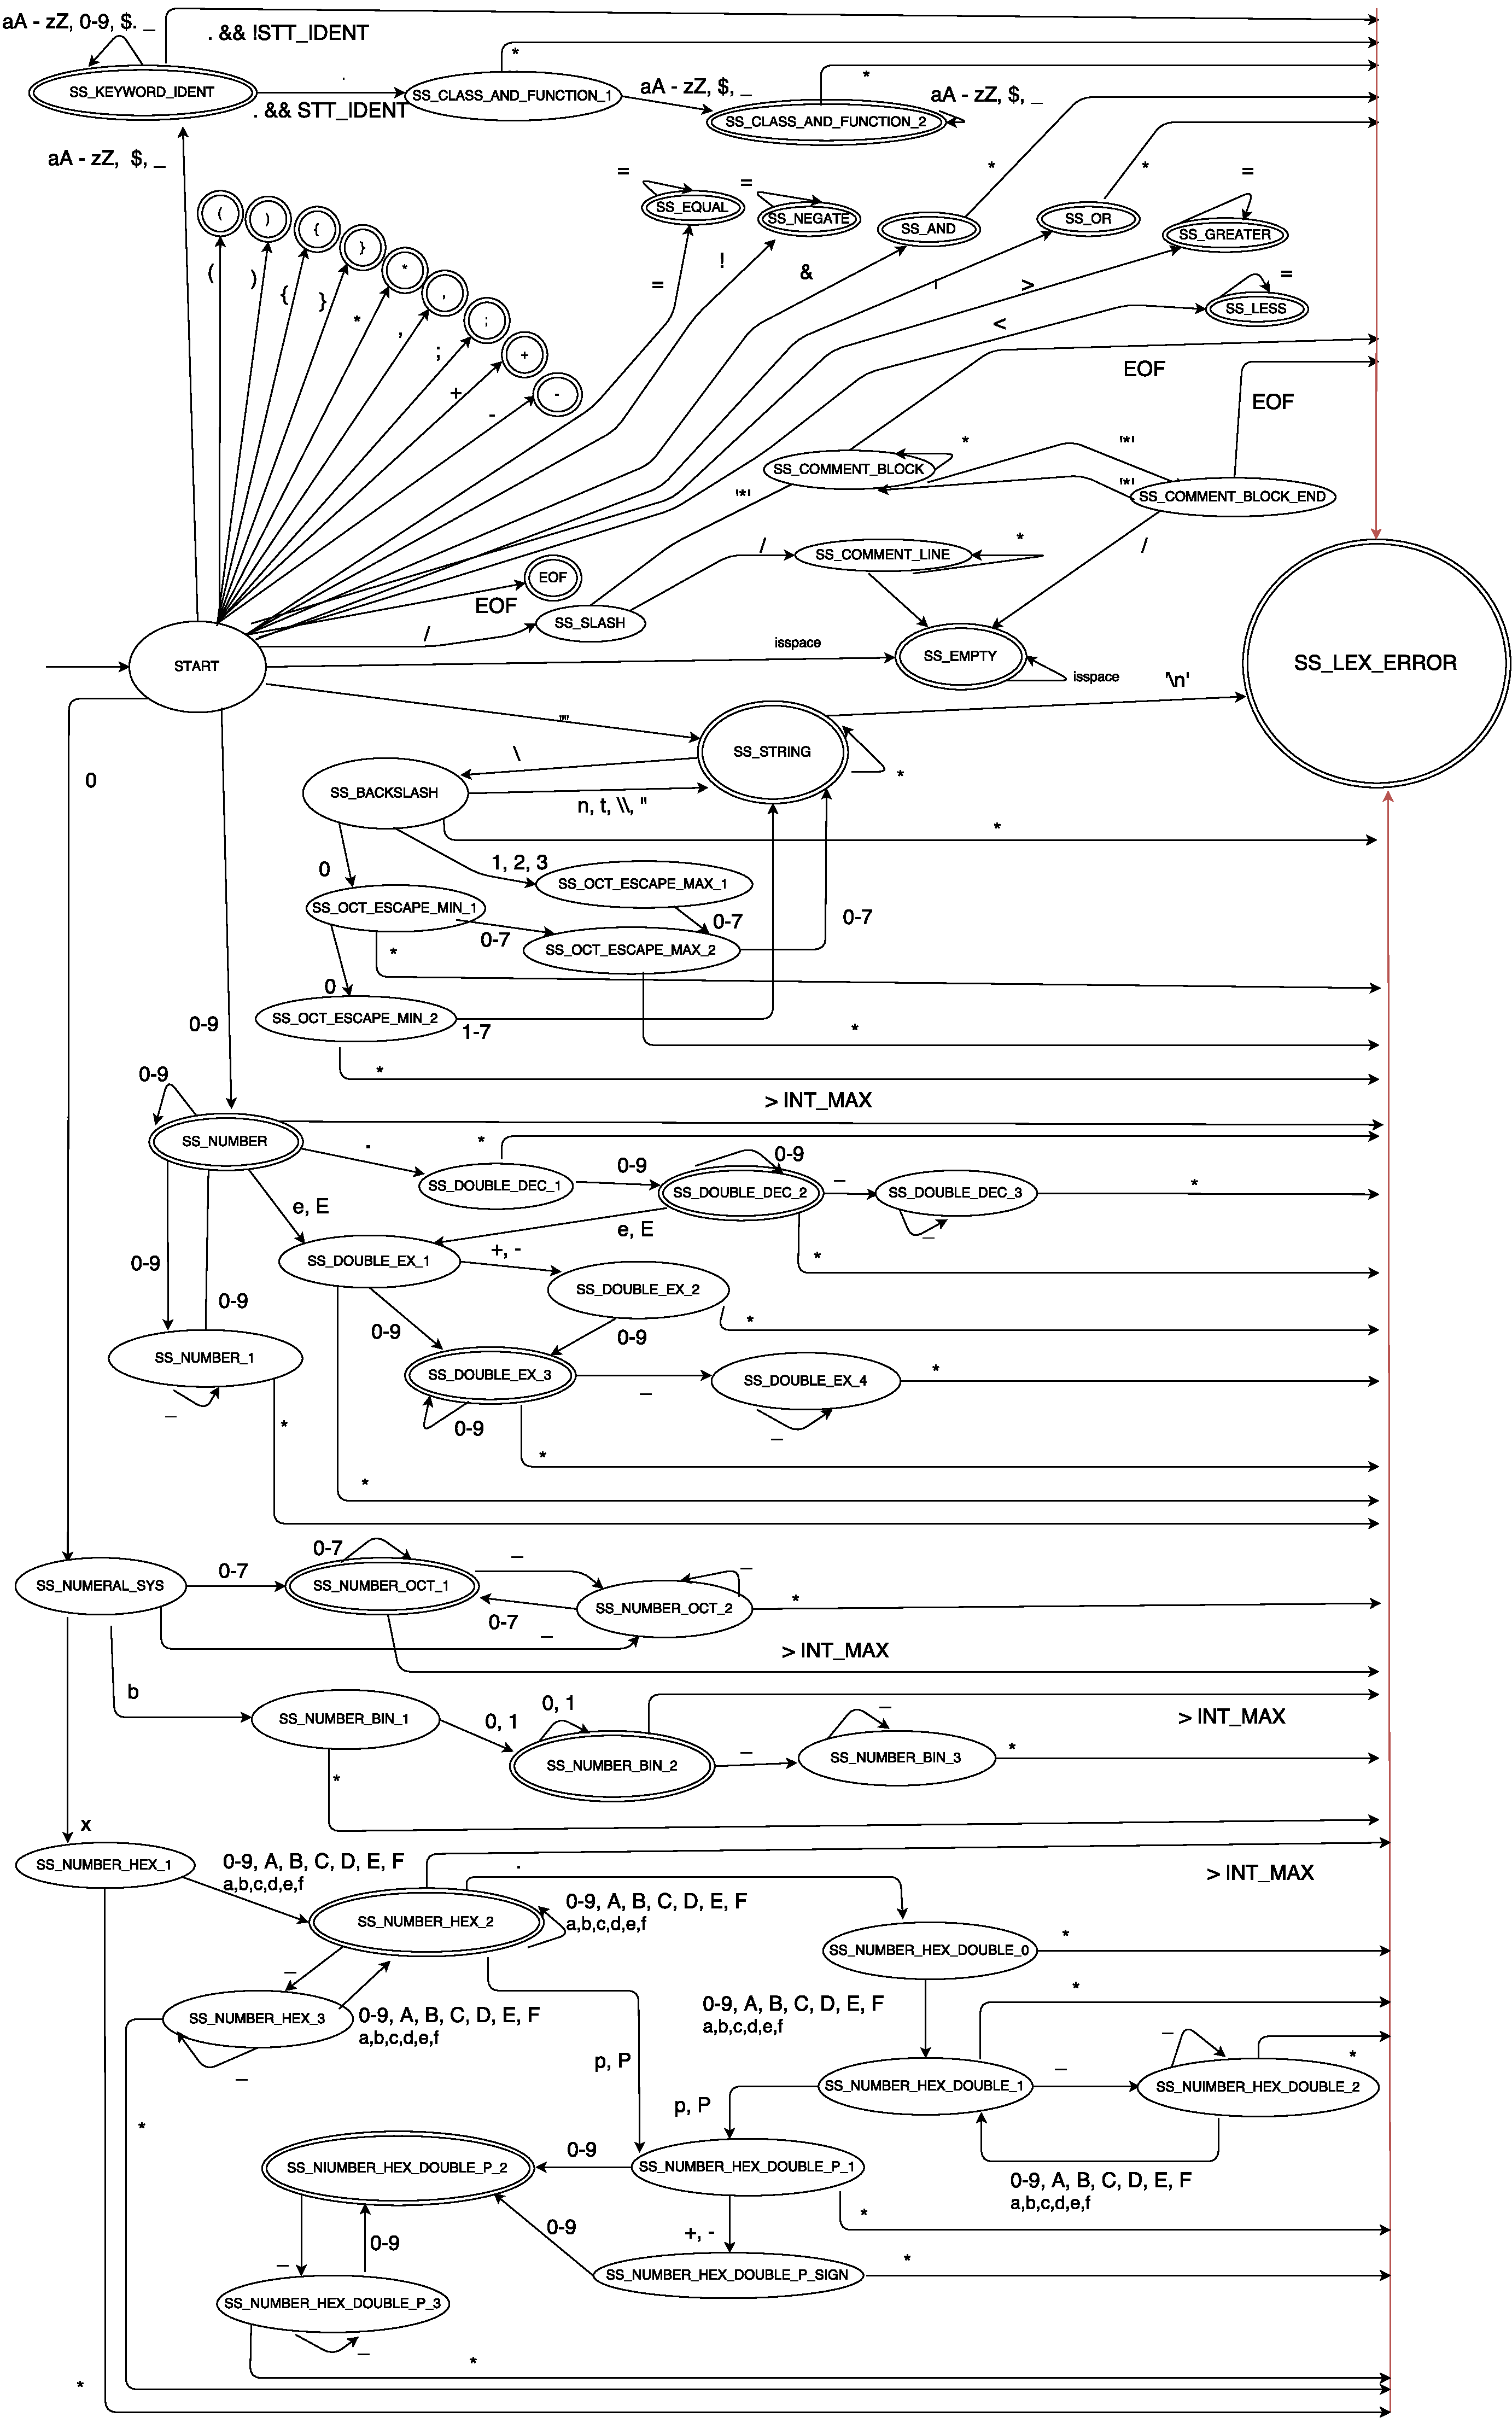
\includegraphics[width=\paperwidth,height=\textheight,keepaspectratio]{ka_scanner_diagram.pdf}
            \end{center}
            
        \subsection{LL gramatika}
        
        \subsection{Precedenčná tabuľka} \label{sec:tab}
        Precedenčná tabuľka slúži na určenie priority tokenov.
        
        \textbf{L} znamená, že token na vrchole zásobníka má menšiu prioritu ako ten vstupný
        
        \textbf{H} naopak znamená, źe je mu nadriadený (má väčšiu prioritu)
        
        \begin{center}
            \begin{tabular}{| c | c | c | c | c | c | c | c | c | c | c | c | c | c |}
            \hline
            SYMBOL & $+$ & $-$ & $*$ & $/$ & $<$ & $>$ & $<=$ & $>=$ & $==$ & $!=$ & $\&\&$ & $||$ & $!$\\
            \hline
            $+$ & H & H & L & L & H & H & H & H & H & H & H & H & L\\
            $-$ & H & H & L & L & H & H & H & H & H & H & H & H & L\\
            $*$ & H & H & H & H & H & H & H & H & H & H & H & H & L\\
            $/$ & H & H & H & H & H & H & H & H & H & H & H & H & L\\
            $<$ & L & L & L & L & H & H & H & H & H & H & H & H & L\\
            $>$ & L & L & L & L & H & H & H & H & H & H & H & H & L\\
            $<=$ & L & L & L & L & H & H & H & H & H & H & H & H & L\\
            $>=$ & L & L & L & L & H & H & H & H & H & H & H & H & L\\
            $==$ & L & L & L & L & L & L & L & L & H & H & H & H & L\\
            $!=$ & L & L & L & L & L & L & L & L & H & H & H & H & L\\
            $\&\&$ & L & L & L & L & L & L & L & L & L & L & H & H & L\\
            $||$ & L & L & L & L & L & L & L & L & L & L & L & H & L\\
            $!$ & H & H & H & H & H & H & H & H & H & H & H & H & L\\
            \hline
            \end{tabular}
        \end{center}
        \subsection{Literatúra}
        \begin{itemize}
            \item Prednašky, skriptá a materiály k predmetu IFJ
        \end{itemize}
        \newpage
    \section{Záver}
    Ak by sme mali zhodnotiť projekt jedným slovom, tak by to asi bolo náročný. Odtestoval nie len naše programátorské schopnosti, ale okrem toho, na ktoré priam dosloval tlačil aj tímové. Celkovo ale hodnotíme projekt pozitívne, lebo nám dal veľa nových skúseností. Tématika projektu bola zaujímavá aj napriek jeho relatívnej obtiažnosti a pomohol nám nie len k lepšiemu chápaniu samotného interpréta, ale aj nám rozšíril znalosti a problematiku týkajúcu sa predmetu IFJ, či aj dokonca ako by približne vyzerala reálna tímová práca v našich potenciálnych zamestnaniach.
    
\end{document}



